\label{ch:experim}

\section{Introducción}\label{header-n0}

Una vez hallada una forma aproximada de representar el sistema de
captación de energía a través del prototipo de columna oscilante de
agua, mediante simulación por ordenador, se procede a idear cómo
desarrollarlo en el laboratorio.

Se realiza una búsqueda por la red de los experimentos que se han
llevado a cabo para el estudio del prototipo OWC, hallando varias formas
para representar su principio de captación de energía. No obstante, para
las características concretas que se desean replicar, no se encontraron
referencias que se adaptasen completamente al caso. Por ello, se
realizan varias modificaciones sobre la marcha y se repitien algunas
fases de la experimentación, para lograr unos valores que se ajusten a
lo deseado.

Tal y como se ha mencionado anteriormente, en el laboratorio de Fluidos
de la escuela de Ingeniería de Bilbao, se dispone de un tanque de olas y
un canal. Ya que no se implementa la generación del oleaje (por su
complejidad a la hora de modelarlo), se decide optar por adaptar el
canal, dejando el tanque para futuros proyectos.

En resumen, se requiere definir una columna de agua en el instante
inicial (como el caso de referencia ``damBreak'' para flujos multifásicos)
para obtener una ola que recorra un canal. En el otro extremo, una
cámara abierta por el fondo, con una chimenea en la parte superior, para
representar el principio de captación del sistema OWC.

El objetivo general será obtener las siguientes variables en el
transcurso del tiempo:

\begin{enumerate}
\def\labelenumi{\arabic{enumi}.}
\item
  Altura del agua en el interior de la cámara.
\item
  Potencia extraida del flujo a la salida de la cámara.
\end{enumerate}

El valor de la potencia, corresponde al caudal que atraviesa por una
turbina WELLS, multiplicado por la perdida de presión a su paso. Debido
a las complicaciones de fabricación e instalación de la turbina a
escala; y que para el análisis computacional sería preciso definirla por
separado, para validar su aerodinámica y el modelo de resolución
aplicado, se sustituye por un diafragma. De esta forma se hallará la
potencia equivalente para el punto de funcionamiento de una turbina en
concreto.

Para hallar el caudal, se descarta la posibilidad de usar un anemómetro,
ya que la escala de velocidades es muy reducida como para que este
aparato aprecie las variaciones del flujo. Además, al tratarse de un
sólo impulso de una ola, no se garantiza la captura del valor máximo.

Sin embargo, la norma \textbf{ISO 5167-2:2003} contempla la medición del
caudal de fluidos mediante dispositivos de presión diferencial
intercalados en conductos en carga de sección transversal circular.
Además, en la \textbf{Parte 2} se describen las \textbf{placas de
orificio}; los detalles sobre la geometria, método de empleo de placas y
medición del caudal. También, se condiciona su aplicación para flujos
subsónicos, monofásicos, de diámetros comprendidos entre 50mm - 1000mm y
números de Reynolds superiores a 5000. Debido a que la salida de aire de
la cámara a la chimenea es como máximo de un diámetro de 30mm, implicará
realizar el experimento para caracterizar los diafragmas que se usarán.

Con todo esto, se adapta el canal, teniendo en cuenta las siguientes
consideraciones y que para el caso particular del canal del laboratório,
sólo se utilizará el montaje para esta ocasión, con lo que no se
realizarán modificaciones permanentes:

\begin{itemize}
\item
  Incluir mecanismo para la apertura de una compuerta. Deberá soportar
  la columna de agua del instante inicial y permitir una apertura lo mas
  limpia y rápida posible.
\item
  Añadir una estructura que actúe como cámara. La anchura quedará
  delimitada por las paredes del canal, se debe permitir la entrada de
  agua por la parte inferior, la salida de aire por la parte superior y
  que soporte el impacto directo de la ola, pudiendo ser anidada al
  fondo del canal.
\item
  Colocar una regla en el canal. Centrada en la cavidad de la cámara
  para captar la media de la altura del agua.
\item
  Acoplar una tubería en la salida de la cámara que haga de chimenea.
  Perforada para poder realizar la lectura de la presión.
\item
  Fabricación de diferentes diafragmas.
\end{itemize}

\section{Fundamentos teóricos}\label{header-n45}

Los instrumentos para medir caudales se llaman \textbf{caudalímetros},
caracterizados por medir el flujo instantáneo, que puede variar de un
momento a otro, \cite{Mataix82}.


Para el ensayo se dispondrá un flujo cerrado, un \textbf{elemento
deprimógeno}, es decir, un elemento que provoca una caída de presión, y
un \textbf{manómetro diferencial} para medir la diferencia de presiones.
Un fluido que circula por un conducto cerrado experimenta una caída de
presión que es funcíon de la velocidad.

Lo característico de una constricción o estrechamiento es que la caída
de presión en la misma \(\Delta h\) es mayor que la pérdida de carga
remanente \(\Delta hr\). Los caudalímetros de constricción más
importantes y ya clásicos en la medida de caudales son: el \textbf{Tubo de
Venturi, las toberas y los diafragmas}.

\subsection{Medida del caudal: Diafragma con sensor de
presión}\label{header-n54}

El diafragma, es una placa con un orificio de diámetro \emph{d}
concéntrico con el eje de la tubería de diámetro \emph{D}. Por su
sencillez de construcción son muy usados para medir caudales tanto en
líquidos como en gases. Resultan muy económicos de instalación, pero
producen una pérdida de carga que es el 50\% de la presión diferencial.

Aplicando Bernoulli para el fluido real, con pérdidas, entre las
secciones 0 y 2:


\[\frac{p_{0}}{\rho g}+z_{0}+\frac{v_{0}^2}{2g}-Hr_{0-2}=\frac{p_{2}}{\rho g}+z_{2}+\frac{v_{2}^2}{2g}\]


Agrupando los términos de presión estática y cotas, la ecuación anterior
queda así:

\[(\frac{p_{0}}{\rho g}+z{0})-(\frac{p_{2}}{\rho g}+z_{2})=h_{0}-h_{2}=Hr_{0-2}+\frac{v_{2}^2}{2g}-\frac{v_{0}^2}{2g}\]

Donde \(h_0-h_{2}\), es la diferencia de alturas piezométricas entre las
secciones 0 y 2.

Las pérdidas \(Hr_{0-2}\) pueden expresarse como fracción de la
velocidad \(v_1\):

\[Hr_{0-2}=\zeta \frac{v_{1}^2}{2g}\]

Donde \(\zeta\), es el coeficiente de pérdidas.

Como el fluido es incompresible, por continuidad se sabe que el caudal
permanece constante, conocidos los diámetros la ecuación de continuidad
queda:

\[v_{0} \frac{\pi D^2}{4}=v_{1} \frac{\pi d^2}{4}=v_{2} \frac{\pi d_{2}^2}{4}\]

Donde \(d_2\) es el diámetro de la \emph{vena contracta}. Por tanto:

\[v_{0}=v_{1}(d/D)^2\]

y

\[v_{2}=v_{1}(d/d_{2})^2\]

Llamando para simplificar:

\[\alpha = d/d_{2}, \beta =d/D\]

Sustituyendo:

\[h_{0}-h_{2}=(\zeta+\alpha^4-\beta^4)\frac{v_{1}^2}{2g}\]

Y despejando:

\[v_1=\frac{1}{\sqrt{\zeta + \alpha ^4-\beta ^4}}\sqrt{2g(h_{0}-h_{2})}\]

\[Q=\frac{\pi d^2}{4}\cdot \frac{1}{\sqrt{\zeta +\alpha ^4-\beta ^4}}\sqrt{2g(h_{0}-h_{2})}\]

\[Q= A_2 \cdot  Cq \sqrt{2g(h_0 -h_2)}\]

Siendo \(A_2\) el área del diafragma y \(C_q\) el coeficiente de caudal
en función de \(m=A_2 /A_1\) y del número de Reynolds.

\subsection{Fluido real por conductos}\label{header-n94}

Un fluido real posee una determinada viscosidad y consecuentemente, la
velocidad de desplazamiento de las partículas de fluido junto a las
paredes del conducto es nula y empieza a aumentar a medida que se aleja
de la pared hasta alcanzar un valor máximo, como se muestra en la
figura \autoref{fig:uconductos}:

\begin{figure}[b]
\centering
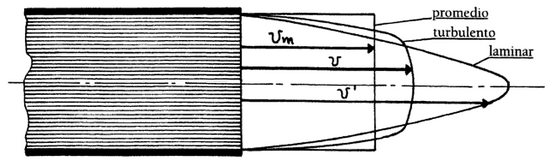
\includegraphics[width=0.8\linewidth]{Uconductos.png}
\caption[Distribución de velocidades]{Distribución de velocidades en un conducto \cite{Luszczewski99}}
\label{fig:uconductos}
\end{figure}

Así mismo, el parámetro primario que afecta a la transición de un flujo
turbulento es el número de Reynolds, en la siguiente tabla se especifica el comportamiento de los flujos según el número de
Reynolds \cite{Mataix82}:

\begin{longtable}[]{@{}cl@{}}
\caption[Comportamiento del flujo según Re]{Comportamientos de los flujos según el número de Re}
%\toprule
\hline
Intervalo & Comportamiento del flujo\tabularnewline
\hline
%\midrule
\endhead
$0 < Re < 1$ & movimiento laminar ``lento'' altamente viscoso\tabularnewline
$1 < Re < 10^2$ & laminar, fuerte dependencia del número de Reynolds\tabularnewline
$10^2 < Re < 10^3$ & laminar, es útil la teoría de capa límite\tabularnewline
$10^3 < Re < 10^4$ & transición a la turbulencia\tabularnewline
$10^4 < Re < 10^6$ & turbulento, moderada dependencia del número de Reynolds\tabularnewline
$10^6 < Re < \infty$ & turbulento, débil dependencia del número de Reynolds\tabularnewline
\hline
%\bottomrule
\end{longtable}


Estos son unos rangos indicativos que pueden variar con la geometría del
flujo, la rugosidad de la superficie y los niveles de fluctuación de la
corriente a la entrada. La mayoría de los análisis versarán sobre flujos
laminares o turbulentos, no siendo recomendable diseñar flujos que
operen en la región de transición.

\section{Descripción del equipamiento}\label{header-n133}

En este apartado se describen brevemente las partes implicadas en el
desarrollo del experimento, así como las adaptaciones que se realizan.

Las pruebas realizadas hasta llegar al caso final se realizan con
materiales reutilizados de otras maquetas del laboratorio, y con la
ayuda de varios técnicos de laboratorio, los cuales colaboraron
prestando material y realizando partes del desarrollo diseñado para la adaptación.

\subsection{Canal}\label{header-n136}

Consta de una bomba para el llenado, \emph{PUMP CPm 132A}, con un caudal
de \emph{20:120 l/min}; y una llave de paso que permitirá ajustar la
condición inicial del nivel del agua. En la imagen \autoref{fig:canal2d} se puede apreciar la imagen del canal al comienzo de los experimentos.

\begin{figure}
\centering
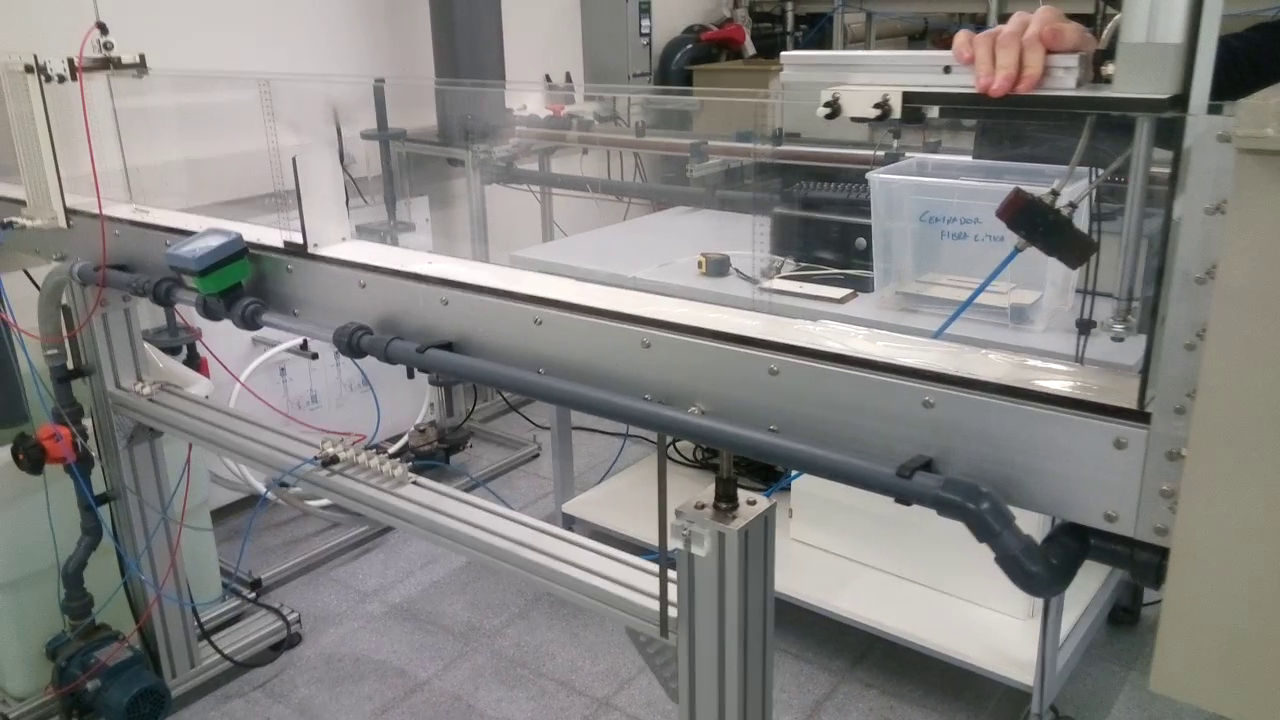
\includegraphics[width=0.8\linewidth]{canal-2018-06-19.png}
\caption{Imagen del canal del laboratorio}
\label{fig:canal2d}
\end{figure}

\subsection{Compuerta}\label{header-n143}

Se fabrica una estructura de madera con un acabado impermeable, que se
anide al canal y a un cilindro hidráulico. Además se pondrán unas juntas
de goma para minimizar las fugas de agua. El pistón, \textbf{serie 453}
de doble vástago, carrera de 160 mm, \textbf{ISO 15552}. Con las
características de este modelo se puede realizar un cálculo rápido para
conocer la fuerza que sería capaz de realizar:

\begin{itemize}
\item
  Presión de operación: 10 bar.
\item
  Diámetro de POM (polyacetal) de 32 mm a 80 mm, luego la fuerza que es
  capaz de realizar:
\end{itemize}

\[
  P_G=10 bar\simeq1000kPa=1000kN/m^2
\]

\[
  F=P_G\cdot A=1000kN/m^2\cdot [(80^2-40^2)\pi]=20,1kN
\]

Así mismo, del cálculo de compuertas planas se obtiene la fuerza que
haría el volumen del agua, considerando el nivel máximo de llenado del
canal, ver \autoref{fig:compuertaplana}:

\begin{figure}
\centering
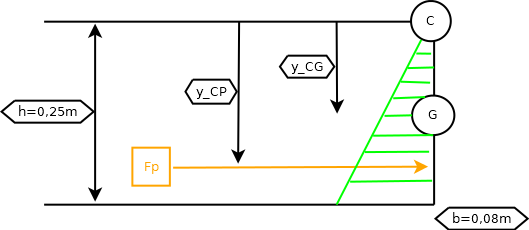
\includegraphics[width=0.8\linewidth]{CompuertaPlana.png}
\caption[Diagrama de presiones]{Diagrama de presiones con la representación de la fuerza máxima ejercida por la columna de agua}
\label{fig:compuertaplana}
\end{figure}

\[
 F_P &= P_G\cdot A=\frac{h}{2}\cdot \gamma \cdot b\cdot h = 9810\frac{N}{m^3}\cdot\frac{0,25^2}{2}m^2\cdot 0,08m = 24,525N
\]

\[
 y_{CP} &= y_{CG}+\frac{I_{XG}}{y_{CG}\cdot A} = \frac{h}{2}+\frac{\frac{1}{12}b\cdot h^3}{\frac{h}{2}\cdot b\cdot h} = \frac{2h}{3}
\]

\[
 \sum M_C &= 0 \xrightarrow{}F_P\cdot y_{CP} = F\cdot 0,16\xrightarrow{}F = 25,547N
\]

Estos resultados no son direcramente comparables, ya que la fuerza del
agua implicaría un momento en el eje del pistón, luego habría que
comprobar el esfuerzo de flexión de dicho eje. No obstante, vista su
capacidad se considera que está sobredimensionado para la función que va
a cumplir, garantizándose también la rápida subida de la compuerta. La estructura diseñada para el pistón se puede apreciar en la fotografía \autoref{fig:piston}.

\begin{figure}[hb]
\centering
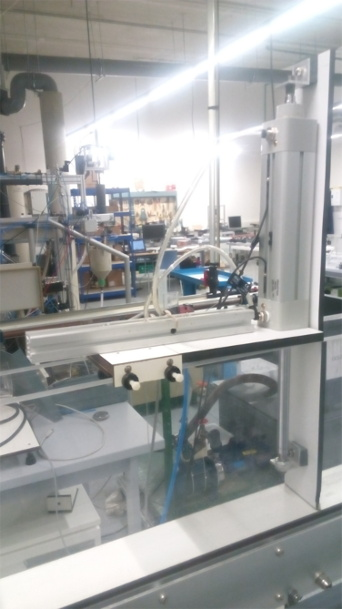
\includegraphics[scale=0.5]{piston.jpg}
\caption[Estructura pistón]{Imagen de la estructura de sujeción para el pistón hidráulico}
\label{fig:piston}
\end{figure}

Asimismo, el accionamiento del pistón se lleva a cabo a través de un programa
desarrollado por un profesor del departamento con la herramienta
\emph{Ni LabVIEW 2015 SPI}. Para ello se conecta el accionamiento
neumático del pistón a una tarjeta de adquisición LabJack U3-Lv (cables
naranjas a la entrada VS y los azules a FIO2 y FIO3); se alimenta
conectado a una placa con una salida de $24V$ y $1,1A$; y por último
se conecta el inyector de aire a presión. En la imagen \autoref{fig:accpiston} se muestra la interacción con el programa para el control de la compuerta desde el ordenador.

\begin{figure}[ht]
\centering
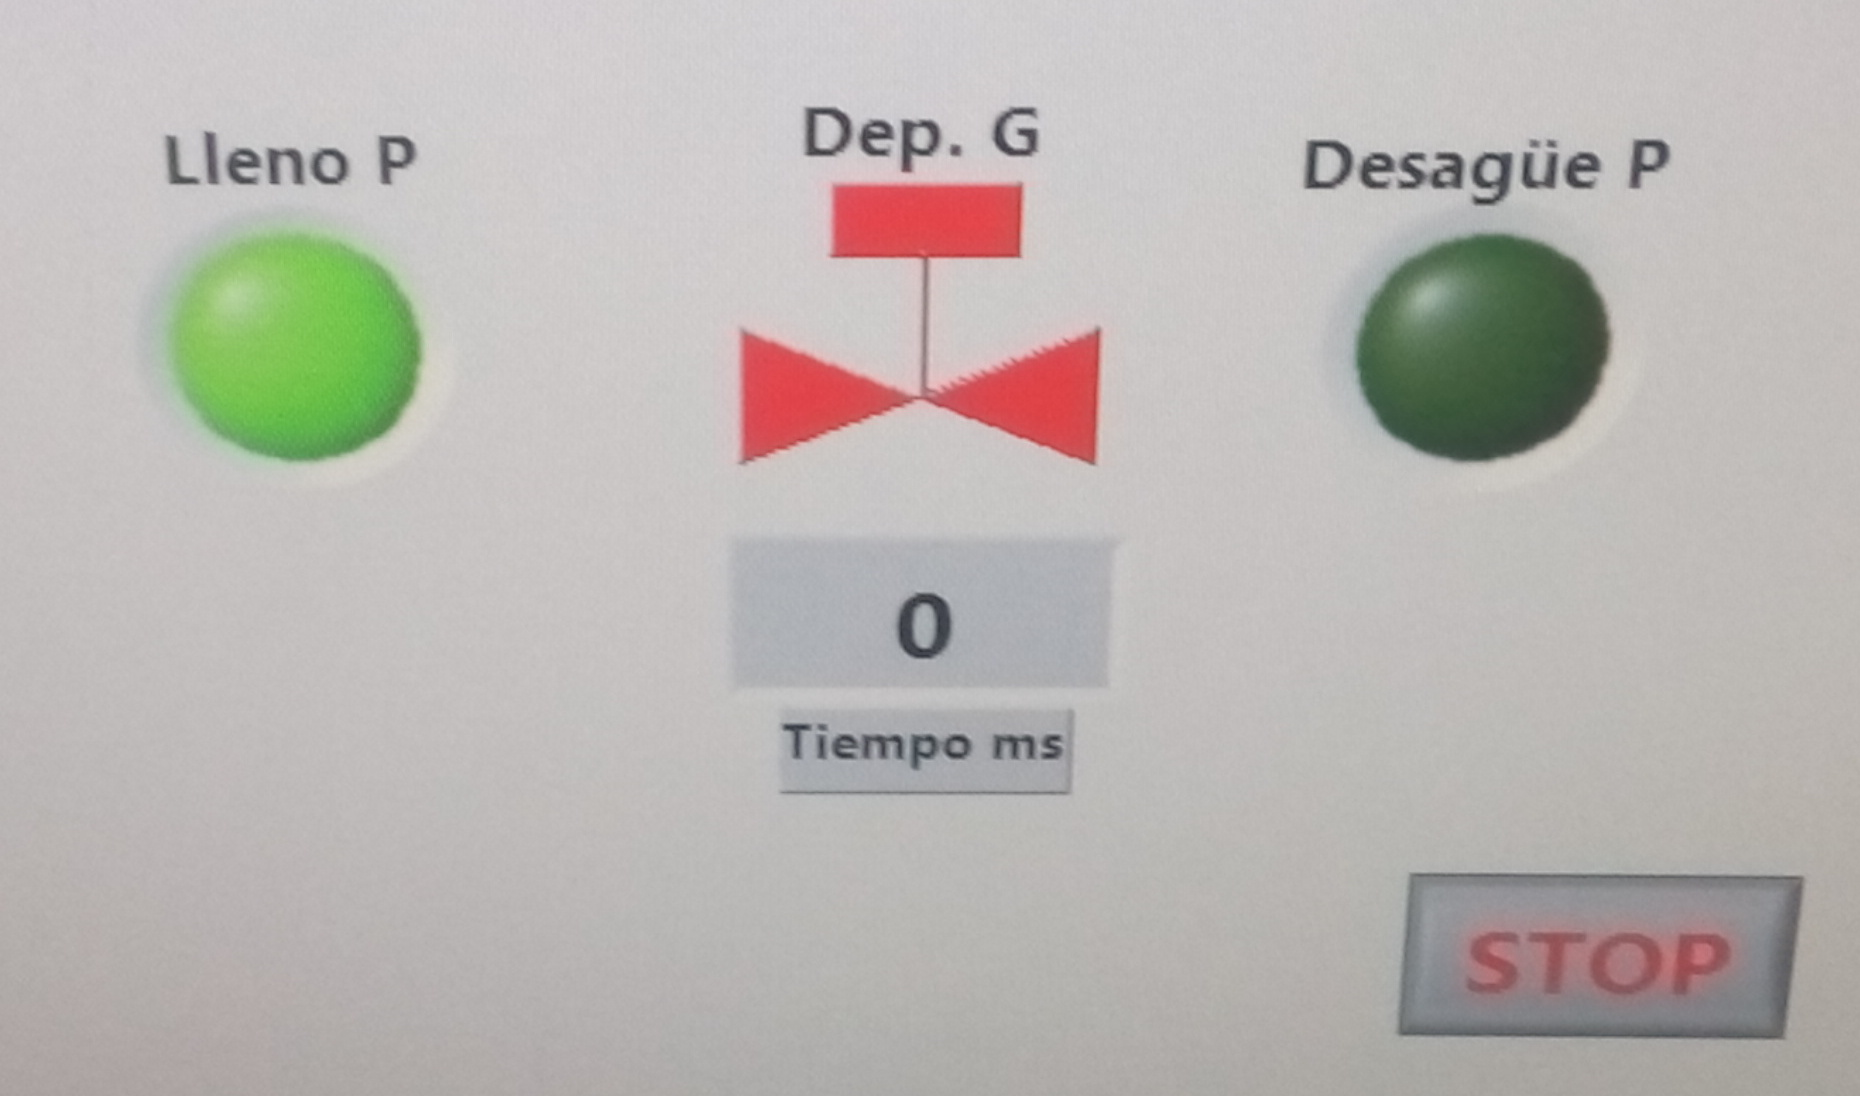
\includegraphics[scale=0.13]{accPiston.jpg}
\caption[Accionado de la compuerta]{Imagen del programa realizado en LabVIEW para el control del pistón hidráulico}
\label{fig:accpiston}
\end{figure}

\subsection{Cámara}\label{header-n602}

Está fabricada con los mismos materiales que la estructura del pistón,
se añaden algunos tacos para facilitar las uniones entre las piezas y
aportar una mayor rigidez a la estructura, la imagen del prototipo se puede apreciar en la \autoref{fig:camara}. La longitud del canal queda
condicionada por los dos puntos de conexión que se disponen en el fondo
del canal, seleccionando el más alejado del origen, para así tener un
mayor recorrido para que el agua colapse y se forme la ola.

Por otro lado, la apertura del paso del agua por el fondo, en un
principio se definió de 25 mm pero como en caso de querer ajustarse a
esa medida habría que reducir la altura total de la cámara, se posiciona
dejando 32 mm de paso.

\begin{figure}
\centering
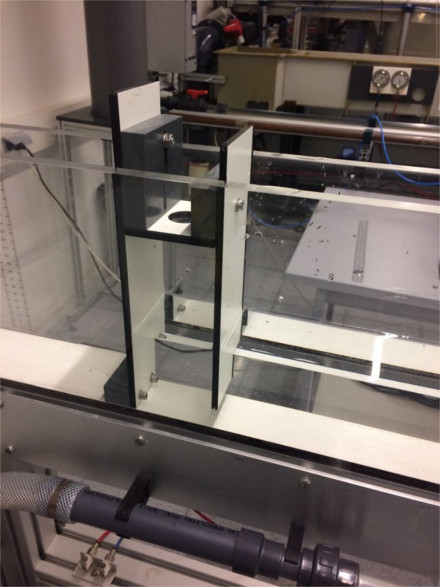
\includegraphics[width=0.6\linewidth]{camara.jpg}
\caption{Imagen del prototipo OWC}
\label{fig:camara}
\end{figure}

\subsection{Chimenea}\label{header-n180}

Se diseña una pieza mediante la impresora 3D para acoplar la tubería,
adaptada en el ensayo de caracterización de los diafragmas que a
continuación se detalla, a la salida de la cámara. Así mismo, se
aprovecha la toma de presión, detallada en el mismo ensayo, para medir
la presión estática del aire dentro de la cámara, dando como resultado la imagen \autoref{fig:prototipo}.

\begin{figure}
\centering
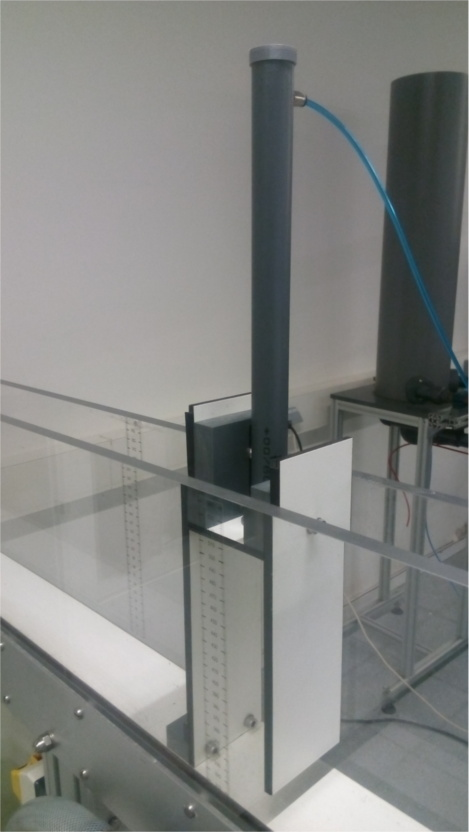
\includegraphics[width=0.45\linewidth]{prototipoOWC.jpg}
\caption[Chimenea]{Fotografía de la chimenea, con el diafragma y la toma de presión}
\label{fig:prototipo}
\end{figure}

El aparato de medida utilizado para hallar la presión es un ``Transductor
de presión diferencial'' marca \emph{Setra}, \textbf{modelo 267}:

\begin{itemize}
\item
  Excitación: 24 VDC/VAC
\item
  Salida: 0-10 VDC
\item
  Serie: 1173078
\item
  Rango: 0-100Pa
\end{itemize}

Se conecta la salida del aparato de medida y algunas resistencias, en
los puertos indicados por un profesor del Dpto., a la misma tarjeta de
adquisición LabJack utilizada para el accionamiento del pistón. A través
de la herramienta \emph{Ni LabVIEW 2015 SPI}, se adapta el programa para
que capture los datos de la presión en el tiempo desde el ordenador. En la imagen \autoref{fig:PTrj} se muestra una captura de la interfaz del programa para el control de las pruebas y las conexiones realizadas en la tarjeta de adquisición. 

\begin{figure}[hb]
\centering
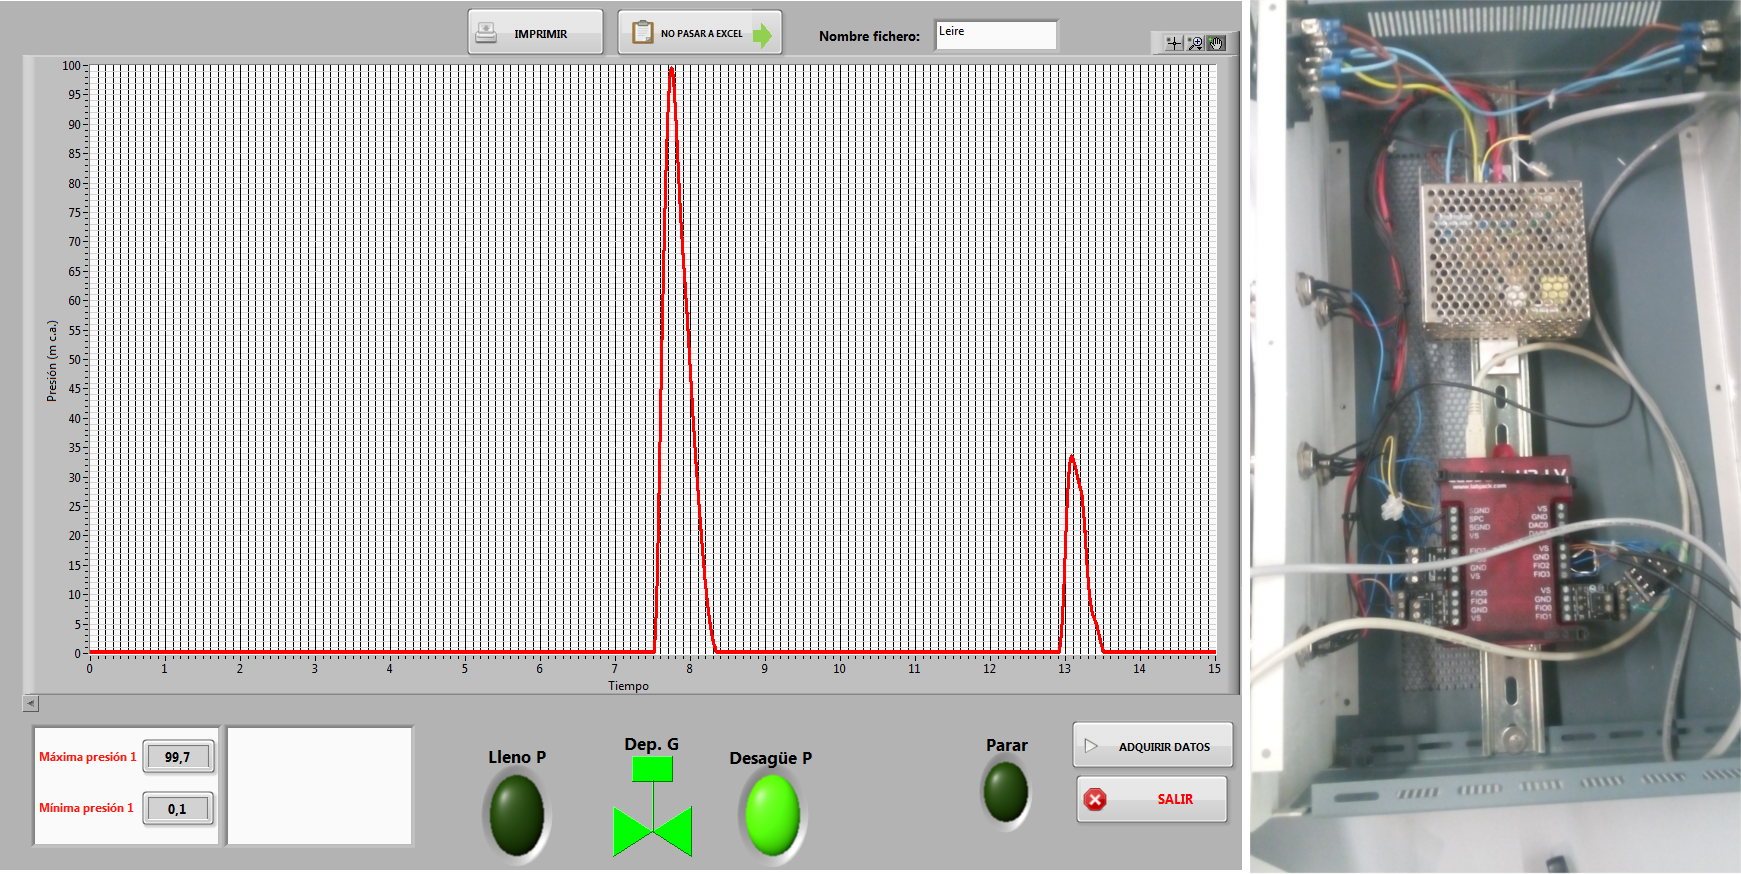
\includegraphics[width=\linewidth]{PTrj.png}
\caption[Adquisición de la presión]{Captura de la señal de la presión y montaje electrónico para la transferencia de las lecturas}
\label{fig:PTrj}
\end{figure}

\subsection{Diafragmas}\label{header-n208}

La normativa \cite{une03} en el apartado sobre el diámetro del orificio
\emph{d}} indica que, éste debe ser en todos los casos mayor que o igual
a \textbf{12,5mm}. Entonces, se toma el valor mínimo contemplado para el
primer modelo de diafragma.

No obstante, como se ha mencionado en la introducción, el diámetro de
salida de la cámara es como máximo de $30mm$, luego no se cumplen las
condiciones (de diámetros \emph{D} comprendidos entre $50mm - 1000mm$)
para tomar un coeficiente de descarga ya definido. Por ello, se
procederá a la caracterización de diferentes diafragmas para hallar los
\emph{Coeficientes de Descarga} correspondientes.

Aparte de esto, dado que el instrumento para medir la presión sólo puede
dar lecturas de hasta $100Pa$, se realiza la simulación del caso para
comprobar a partir de que diámetro se supera dicha presión. Comprobando
que para el diámetro de 12,5mm se superan los $120Pa$, entonces, se decide
aumentar dicho diámetro y realizar el experimento para los diafragmas:
$[13-14-15,5-16] mm$. Estas piezas se frabrican a partir de una
impresora 3-D y se diseñan mediante OpenSCAD, en la imagen \autoref{fig:d13} se muestra el modelo desde el programa mencionado además del boceto con las dimensiones introducidas.

\begin{figure}
\centering
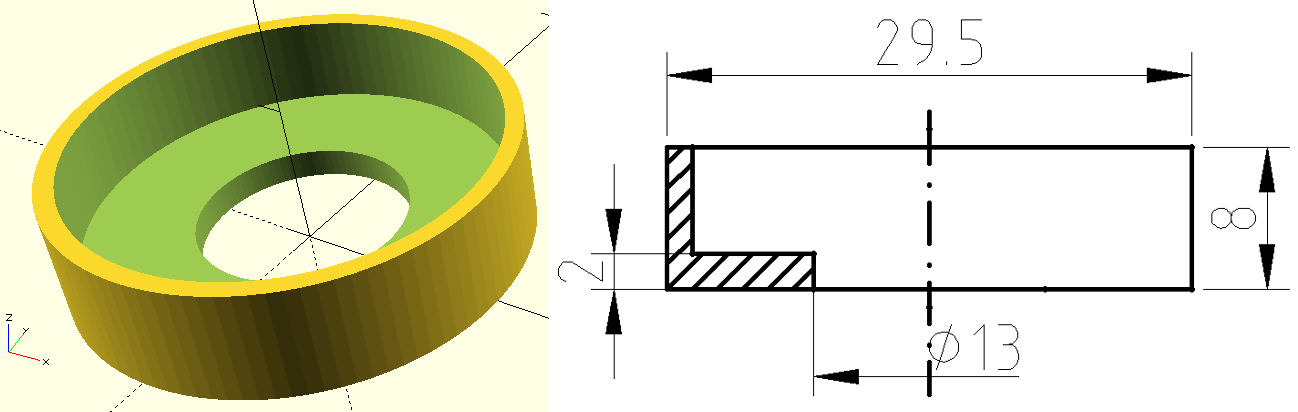
\includegraphics[width=0.9\linewidth]{d13.png}
\caption[Modelo diafragma]{Captura del modelo desde OpenSCAD y boceto del diseño}
\label{fig:d13}
\end{figure}

\subsection{Impresora 3D}\label{header-n221}

Modelo \textbf{Prusa i3}, características:

\begin{itemize}
\item
  Tipo de plástico utilizado: \textbf{PLA}, hecho a partir de materiales
  orgánicos y renovables, en el proceso de impresión se usa un diámetro
  de boquilla (\emph{nozzle}) de $0,4 mm$, el diámetro del filamento de
  $1,75 mm$, anchura de capa de $0,2 mm$ (calidad normal) y densidad de
  relleno (\emph{infill}) de 15\%. Aunque se trate de mejorar la
  configuración de impresión, este material crea un paso visible entre
  las capas, luego el acabado superficial suele ser rugoso, pero es
  bastante resistente, apropiado para el prototipado y perfección de
  diseños finales.
\item
  Margen de compensación: Para que las medidas resulten exactas a las
  establecidas y que las piezas encajen correctamente, se aumenta la
  dimensión de los diámetros interiores 0,4mm.
\item
  Margen de impresión: $x = 215 mm$, $y = 210 mm$, $z = 180 mm$.
\item
  Formato de entrada: para definir las características de impresión se
  utiliza el software CURA del que se obtiene un archivo \emph{.gcode}.
  Además, este programa necesita que los modelos se importen en formato
  STL y de entre las alternativas existentes, se selecciona el software
  paramétrico OpenSCAD.
\end{itemize}

\section{Caracterización de diafragmas}\label{header-n239}

Tal y como se ha mencionado en el apartado de \ref{header-n208} Diafragmas, el
diámetro de salida de flujo de aire por la chimenea es como máximo de
30mm, por lo que no entra dentro de las condiciones contempladas por la
normativa para aplicar un \emph{coeficiente de caudal} normalizado.

\subsection{Objeto}\label{header-n246}

La elección de un medidor de flujo se ve afectada por la exactitud
requerida, el intervalo de medición, el costo, la complicación, la
facilidad de lectura o reducción de datos, así como la vida de servicio.
En este caso se trata de hallar la forma más simple para llevar a cabo este
experimento, reutilizando los materiales disponibles en el laboratorio e
incluso, prestado por otros departamentos.

Cuando se tiene una obstrucción en un tubo, aparece un diferencial de
presión. Esta caída de presión se puede correlacionar con la descarga
mediante una calibración, y después se puede utilizar la curva
presión-descarga para determinar la descarga leyendo la presión
diferencial. Para ello se necesitará un flujo estable, así la ecuación
de Bernoulli y la ecuación de continuidad servirán para determinar la
descarga, \cite{Mataix82}.

En el caso del diafragma, las líneas de corriente convergen para formar
un área de flujo mínimo, ``vena contracta'', debido a que se desconoce
este área, conviene usar el área de la obstrucción de diámetro \emph{d}.
Para considerar el efecto de la contracción y un coeficiente de
velocidad, se introduce un \textbf{coeficiente de descarga C}. Además,
se emplea un \textbf{coeficiente de flujo K} que considera el
coeficiente de descarga y la relación de áreas o diámetros de la
obstrucción y la tubería. Un análisis dimensional revelaría que \emph{C}
y \emph{K} dependen del número de Reynolds.

La presión estática en la tubería se medirá instalando un
\textbf{piezómetro}; con el \textbf{tubo de Prandtl} se obtendrá la
diferencia entre la presión total y la estática, y de ahí obtener la
presión dinámica. Entonces, será posible hallar la velocidad del flujo y
con ello, el caudal, el coeficiente de descarga y el número de Reynolds
serán valores conocidos.

\subsection{Métodos desarrollados}\label{header-n257}

\subsubsection{Definición}\label{header-n258}

En un comienzo se trató de obtener el \emph{Coeficiente de Descarga} a
partir de las maquetas de ensayo dispuestas en el laboratorio colocando
a la salida del tubo de aire una tapa con el diafragma de 12,5mm
fabricado con la impresora 3-D y realizado desde OpenSCAD.

Las primeras mediciones se realizan en un tubo horizontal de
\textbf{113mm} de diámetro interior, con un ventilador de 12V DC 0,09A,
al que se le pueden controlar las rpm. El flujo se encuentra una
oposición muy brusca al reducirse hasta 12,5mm el diámetro de la salida;
por ello, se produce un flujo muy turbulento y las mediciones de la
presión dinámica resultan erróneas, a pesar de tratar de resolver el
error aumentando la longitud de la tubería de salida.

Se prosigue con la segunda prueba, realizada en un tubo de díámetro más
pequeño, de \textbf{54mm}, con un ventilador centrífugo y donde el flujo
de aire cambia de dirección 90º. Sin embargo, las mediciones de la
\emph{Pd}, hallada con el tubo de Prandtl, como en el caso anterior,
seguian siendo demasiado inestables.

Para evitar estos rebotes del flujo, se procede a reducir la relación de
diametros y, así, suavizar el paso del flujo por el diafragma. Se
utiliza una tubería de diámetro interior \textbf{19,6mm} y un ventilador
VEN003 de 12vcc, con un caudal de 8,53CFM ($0,004m^3/s$). En primer lugar
se trató de medir el caudal con un anemómetro, pero la resistencia que
oponen los álabes frente al poco caudal de aire, hace que este
instrumento no sea el más apropiado para apreciar variaciones pequeñas
en la velocidad de flujo. Por tanto, se decide colocar un tubo de
Prandtl, como para los casos anteriores. Se siguen los pasos de la
normativa para diseñar las partes de unión entre la tubería y los
diferentes aparatos.

En la imagen \autoref{fig:M1M2M3M4} se resumen los tres casos experimentados en un primer momento de forma insatisfactoria.
\begin{figure}[hb]
\centering
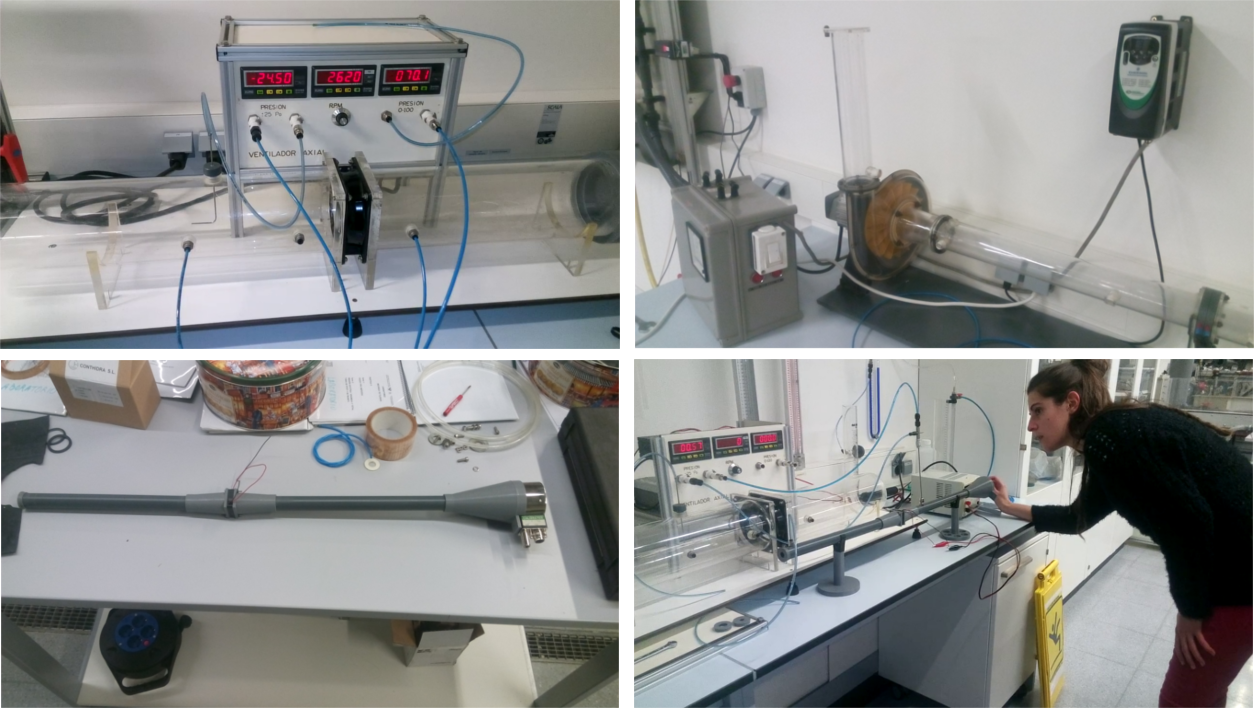
\includegraphics[width=\linewidth]{M1M2M3M4.png}
\caption[Métodos fallidos realizados]{Métodos fallidos realizados, de izquierda a derecha y de arriba abajo M1, M2, M3 y M4}
\label{fig:M1M2M3M4}
\end{figure}

\subsubsection{Consideraciones para el diseño: Norma UNE-EN ISO 5167-2.03H}\label{header-n277}

\textbf{Placas de orificio}

En la norma \cite{une03}, se describe el diafragma como, la parte
de la placa dentro del conducto, la cual, debe ser circular y
concéntrica con el eje del conducto. Las caras de la placa deben ser
planas y paralelas.

Además, el diámetro \emph{d} debe ser en todos los casos mayor que o
igual a \textbf{12,5 mm} y la relación de diámetros \(\beta =d/D\), debe
ser siempre mayor que o igual a \textbf{0,10}, y menor que o igual a
\textbf{0,75}. Siendo \emph{D} \textbf{19,6mm} la relación de diámetros
queda dentro del rango con un valor de \textbf{0,64}.

También se definen los requisitos a cumplir cuando se
trabaja con \textbf{placas bidireccionales}, donde la placa de orificio
se utilizará con flujos opuestos, como es el caso a estudio:

 a) la placa no debe ser biselada,

 b) las dos caras deben cumplir con las especificaciones para la cara
aguas arriba. Es decir, la placa puede
considerarse plana cuando el máximo huelgo entre la placa y el canto
recto de longitud \emph{D}, tendido a través de cualquier diámetro de la
placa, es menor de \textbf{0,005(D-d)/2}, es decir, la pendiente es
menor de \textbf{0,5\%} cuando la placa es examinada antes de
intercalarla dentro de la línea de medida,

 c) el espesor \emph{E} de la placa debe ser igual al espesor \emph{e}
del orificio, comprendido entre \textbf{0,005D y 0,02D}
\textbf{(0,098 a 0,392mm)}, además la diferencia entre los valores de e,
medidos en cualquier punto del orificio, no debe ser mayor de
\textbf{0,001D} \textbf{(0,0196mm)},

 d) los dos cantos del orificio deben cumplir con las especificaciones
para el canto aguas arriba (apartado 5.1.7). El canto aguas arriba no
debe tener cantos rotos o protuberancias, debe estar bien marcado, se
considera así si el radio del canto no es mayor de \textbf{0,0004d}
\textbf{(0,005)}.

\textbf{Tomas de presión}

Para cada placa de orificio, debe instalarse al menos una toma de
presión aguas arriba y una toma de presión aguas abajo a \textbf{D y
D/2}. Como el diafragma se coloca en un extremo de la
tubería solo se considera la medida aguas arriba, ya que aguas abajo se
tiene la presión atmosférica.

\begin{itemize}
\item
  \emph{Aguas arriba}: $l_1 = D \pm 0,1D$ \textbf{= \textbf{21,56mm}}
\item
  \emph{Aguas abajo}: $l_2 = 0,5D \pm 0,01D$ \textbf{= 9,996mm}
\end{itemize}

El eje de la toma debe formar con el eje del conducto un ángulo tan
próximo a 90º como sea posible. El orificio debe ser circular en el
punto de perforación, los cantos deben estar al ras de la superficie
interna de la pared del conducto y con acabado superficial lo más
marcado posible. El diámetro de las tomas de presión debe ser menos de
$0.13D$ (\textbf{2.548 mm}), y menor de $13 mm$. Los ejes de las tomas de
presión pueden situarse en cualquier plano axial de la tubería.

\textbf{Requisitos de instalación}

Asimismo, en la normativa se especifican las \textbf{longitudes rectas mínimas}
aguas arriba y aguas abajo para instalaciones \textbf{entre diversos
accesorios y la placa de orificio}:

\begin{itemize}
\item
  Estas longitudes para los accesorios especificados en la instalación,
  sin acondicionadores del flujo, se muestran en la tabla 3, de la normativa.
\item
  Cuando no se utiliza un acondicionador del flujo, las longitudes
  especificadas en la normativa deben considerarse como los valores
  mínimos. En particular, para trabajos de investigación y calibración,
  se recomienda que los valores aguas arriba especificados en la tabla 3 \cite{une03}
  se incrementen por al menos un factor de 2, para minimizar la
  incertidumbre de medida.
\item
  Cuando las longitudes rectas utilizadas son iguales a o mayores que
  los valores especificados para
  ``incertidumbre adicional cero'', no es necesario aumentar la
  incertidumbre del coeficiente de descarga para tener en cuenta el
  efecto de la instalación particular.
\end{itemize}

Para el caso particular del ensayo, se debe adecuar el diámetro del
ventilador al diámetro del tubo \emph{D}, para ello se colocará un
reductor a una distancia de la placa de orificio, tomando el valor de la
relación entre diámetros 0,67 (\textbf{0,64}), con ``incertidumbre
adicional cero'':

\begin{itemize}
\item
  \emph{Aguas arriba}: $L_1 = 12\times D$ = \textbf{235,2 mm}
\item
  \emph{Aguas abajo}: $L_2 = 7\times D = 137,2 mm$
\end{itemize}

Para que el reductor cumpla una instalación aceptable deberá fabricarse
con una relación de $2D$ a $D$ (\textbf{38mm a 19,6mm}) sobre una longitud
de $1,5D$ a $3D$ (29,4\textless{}\textbf{50mm}\textless{} 58,8).

\textbf{Acondicionadores del flujo}

Un acondicionador del flujo (apartado 6.3) puede utilizarse para reducir
longitudes rectas aguas arriba, para el caso particular a ensayar, se
utilizará para prevenir turbulencias aguas arriba. Dado que el diseño
del ventilador produce un aire muy elicoidal (diseñados para disipar el
calor, consta de un diámetro de eje grande en proporción al total), como
para provocar vórtices en el flujo.

Los acondicionadores del flujo sin patentar, que han cumplido el ensayo
de conformidad de la Norma ISO 5167-1, son el enderezador del flujo de
haz de 19 tubos (1998) y el acondicionador del flujo placa Zanker. Ya
que no se dispone de un diámetro de tubo de gran dimensión, se fabrica
el de 8 paletas, patentado y descrito en el Anexo B.

El espesor de la pared debe ser menor que $0,025D$(\textbf{0,49mm}), para
que exista una igualdad en cuanto a uniformidad, diámetro exterior y
espesor de pared. Además la longitud indicada será de 2D (\textbf{39,2mm}) o 3D.

\begin{itemize}
\item
  Instalación aguas abajo de cualquier accesorio: En este caso, tras el
  reductor del ventilador, se tomará la medida para el enderezador del
  flujo de haz de 19 tubos, de modo que la distancia entre el extremo
  aguas abajo del acondicionador y la placa de orificio, sea igual a $13D
  \pm 0,25D (254,8 \pm 4,9 = \textbf{259,7 mm})$.
\end{itemize}

\subsubsection{Datos y lecturas}\label{header-n345}

A continuación, se describen los resultados obtenidos del último método
mencionado. El cual, se dispone con una fuente de alimentación para
alimentar el ventilador VEN003, un tubo de Prandtl para medir la presión
dinámica y un piezómetro colocado aguas arriba del diafragma.

Se conecta la salida superior del tubo de Prandtl, de donde se obtiene
la presión total, al lado derecho del aparato de medición de la presión;
y la otra salida (colocada en horizontal), se conecta a la izquierda
para que el intrumento de medición realice la resta de:
\(P_d =P_T - P_e\). El valor de esta variable es muy pequeño, luego se
mide entre el rango \(\pm 25Pa\).

Por otra parte, el valor de la diferencia de presiones a un lado y al
otro del diafragma, se obtiene conectando esta salida al lado derecho
del aparato de medida, dejando el lado izquierdo abierto a la atmósfera.
La presión estática aguas arriba del diafragma también resulta muy
pequeña, luego se halla del mismo rango de medida que para el caso
anterior.

Una vez dispuesto el montaje, se prepara una ficha de excel con los
siguientes datos:

\begin{itemize}
\item
  \(\rho _ {\text{aire}} = 1,2 kg/m^3\)
\item
  \(\nu _ {\text{aire}}=1,8 \cdot 10^{-5} \frac{N\cdot s}{m^2}\)
\item
  \(g=9,81 m/s^2\)
\item
  $D=0,0196 m$
\item
  \(d=0,013m\)
\item
  \(\beta =d/D= 0,66\)
\item
  \(A_D = 3,01719 \cdot 10^4 m^2\)
\item
  \(A_d = 1,32732 \cdot 10^4 m^2\)
\end{itemize}

Aparte de esto de define una tabla para anotar las mediciones y
calcular:

\begin{itemize}
\item
  La \textbf{velocidad}, se obtiene de la presión dinámica, medida con
  el tubo de Prandtl, siendo:

  \[P_d=\frac{v^2}{2}\cdot \rho \to v=\sqrt{\frac{2\cdot P_d}{\rho}}\]
\item
  El \textbf{caudal}, con el valor de la velocidad conocido, se
  multiplica por el área del tubo \emph{D} y, así, hallar el caudal de
  flujo de aire que circula por el interior:

  \[Q=v\cdot A_D\]
\item
  \textbf{Coeficiente de descarga}, de la ecuación del apartado \autoref{header-n54} se aunan los
  términos constantes en un nuevo parámetro \emph{K}, quedando la
  siguiente ecuación:

  \[Q=K\sqrt{\Delta P} = K\cdot \sqrt{P_1-P_2}\]

  siendo \(P_2\), la presión atmosferica, su valor corresponde a cero
  por estar trabajando con presiones manométricas, entonces:

  \[K=\frac{Q}{\sqrt{P_1}}\]
\item
  El \textbf{número de Reynolds} se obtiene del valor calculado de la
  velocidad, a partir de la medición con el tubo de Prandtl; luego, se
  multiplica por el diámetro del tubo y se divide por la viscosidad del
  flujo de aire:

  \[Re= \frac{v\cdot D}{\nu _{aire}}\]
\end{itemize}

El flujo máximo que se consigue mediante este método, queda limitado por
la máxima tensión que el ventilador es capaz de aguantar. Con lo cual,
se irá reduciendo la tensión hasta que la medida de la presión se
aproxime a cero, en la tabla \autoref{tab:tablaM4} se resumen las lecturas y los valores de las variables calculadas a partir de estas.

\begin{table}[hb]
\centering
\caption{Resultados del Método 4}
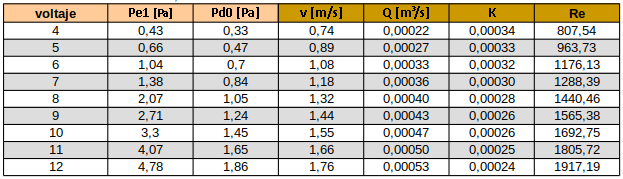
\includegraphics[width=0.8\linewidth]{tablaM4.png}
\label{tab:tablaM4}
\end{table}

Finalmente se realiza una gráfica (x-y) de los valores del coeficiente
de descarga equivalente respecto el número de Reynolds, para un valor de
\(m=A_2/A_1=0,41\), ver \autoref{fig:grafM4}.

\begin{figure}[ht]
\centering
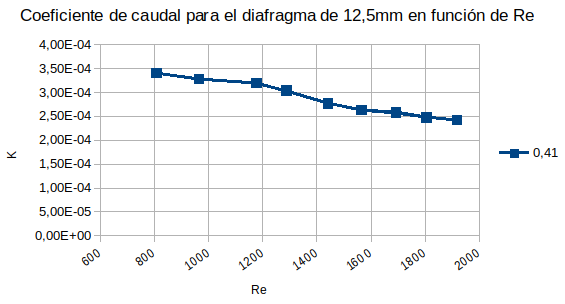
\includegraphics[width=0.7\linewidth]{grafM4.png}
\caption[Caracterización del diafragma $12,5mm$]{Caracterización del diafragma $12,5mm$, representación del coeficiente de descarga}
\label{fig:grafM4}
\end{figure}

\subsubsection{Conclusiones}\label{header-n423}

A partir de esta gráfica se obtiene el \emph{coeficiente de descarga
equivalente} para cierto valor de \emph{Re} y para los díametros del
tubo de 19,6mm y del diafragma de 12,5mm. Junto con esto, si se toma el
valor de la presión aguas arriba del diafragma del ensayo del canal se
podrá obtener el caudal y la potencia de la siguiente manera:

\begin{itemize}
\item
  De la ecuación despejada en el subapartado \ref{header-n345}: \(Q=K\sqrt{P_1}\)
\item
  El resultado de la potencia se obtiene de sustituir la ecuación
  anterior de la siguiente forma:
\end{itemize}

\[Pot= \rho g Q H = \Delta P \cdot Q=P_1\cdot Q=P_1K\sqrt{P_1}=K\cdot P_1^{3/2}\]

No obstante, tras simular el caso se obtienen los siguientes valores,
para el máximo valor de la velocidad de flujo:

\begin{itemize}
\item
  \(U=5,22 m/s\)
\item
  \(P_d=16,37Pa\)
\item
  \(Q=0,00158m^3/s\)
\item
  \(Re=5684,71\)
\end{itemize}

Luego, el método empleado no sirve, ya que no se alcanzan los valores de
\emph{Re} que se tendrán en el ensayo final. Se decide modificar la
forma en la que se genera el flujo de aire, concluyendo que para evitar
los errores anteriores, lo más eficaz será conectar un inyector de aire
a presión. De este modo se podrá aumentar la velocidad del flujo, lo que
afectará a un incremento en el número de \emph{Re}.

\subsection{Método final}\label{header-n453}

\subsubsection{Definición}\label{header-n454}

Reutilizando las partes ya creadas para los anteriores experimentos, se
realiza una pieza para que encaje con la salida del inyector de aire a
presión mediante OpenSCAD. Además, en el tubo de inyección se coloca un
regulador de caudal para obtener diferentes caudales de aire, ver imagen de la maqueta \autoref{fig:M5inyector}.

\begin{figure}[hb]
\centering
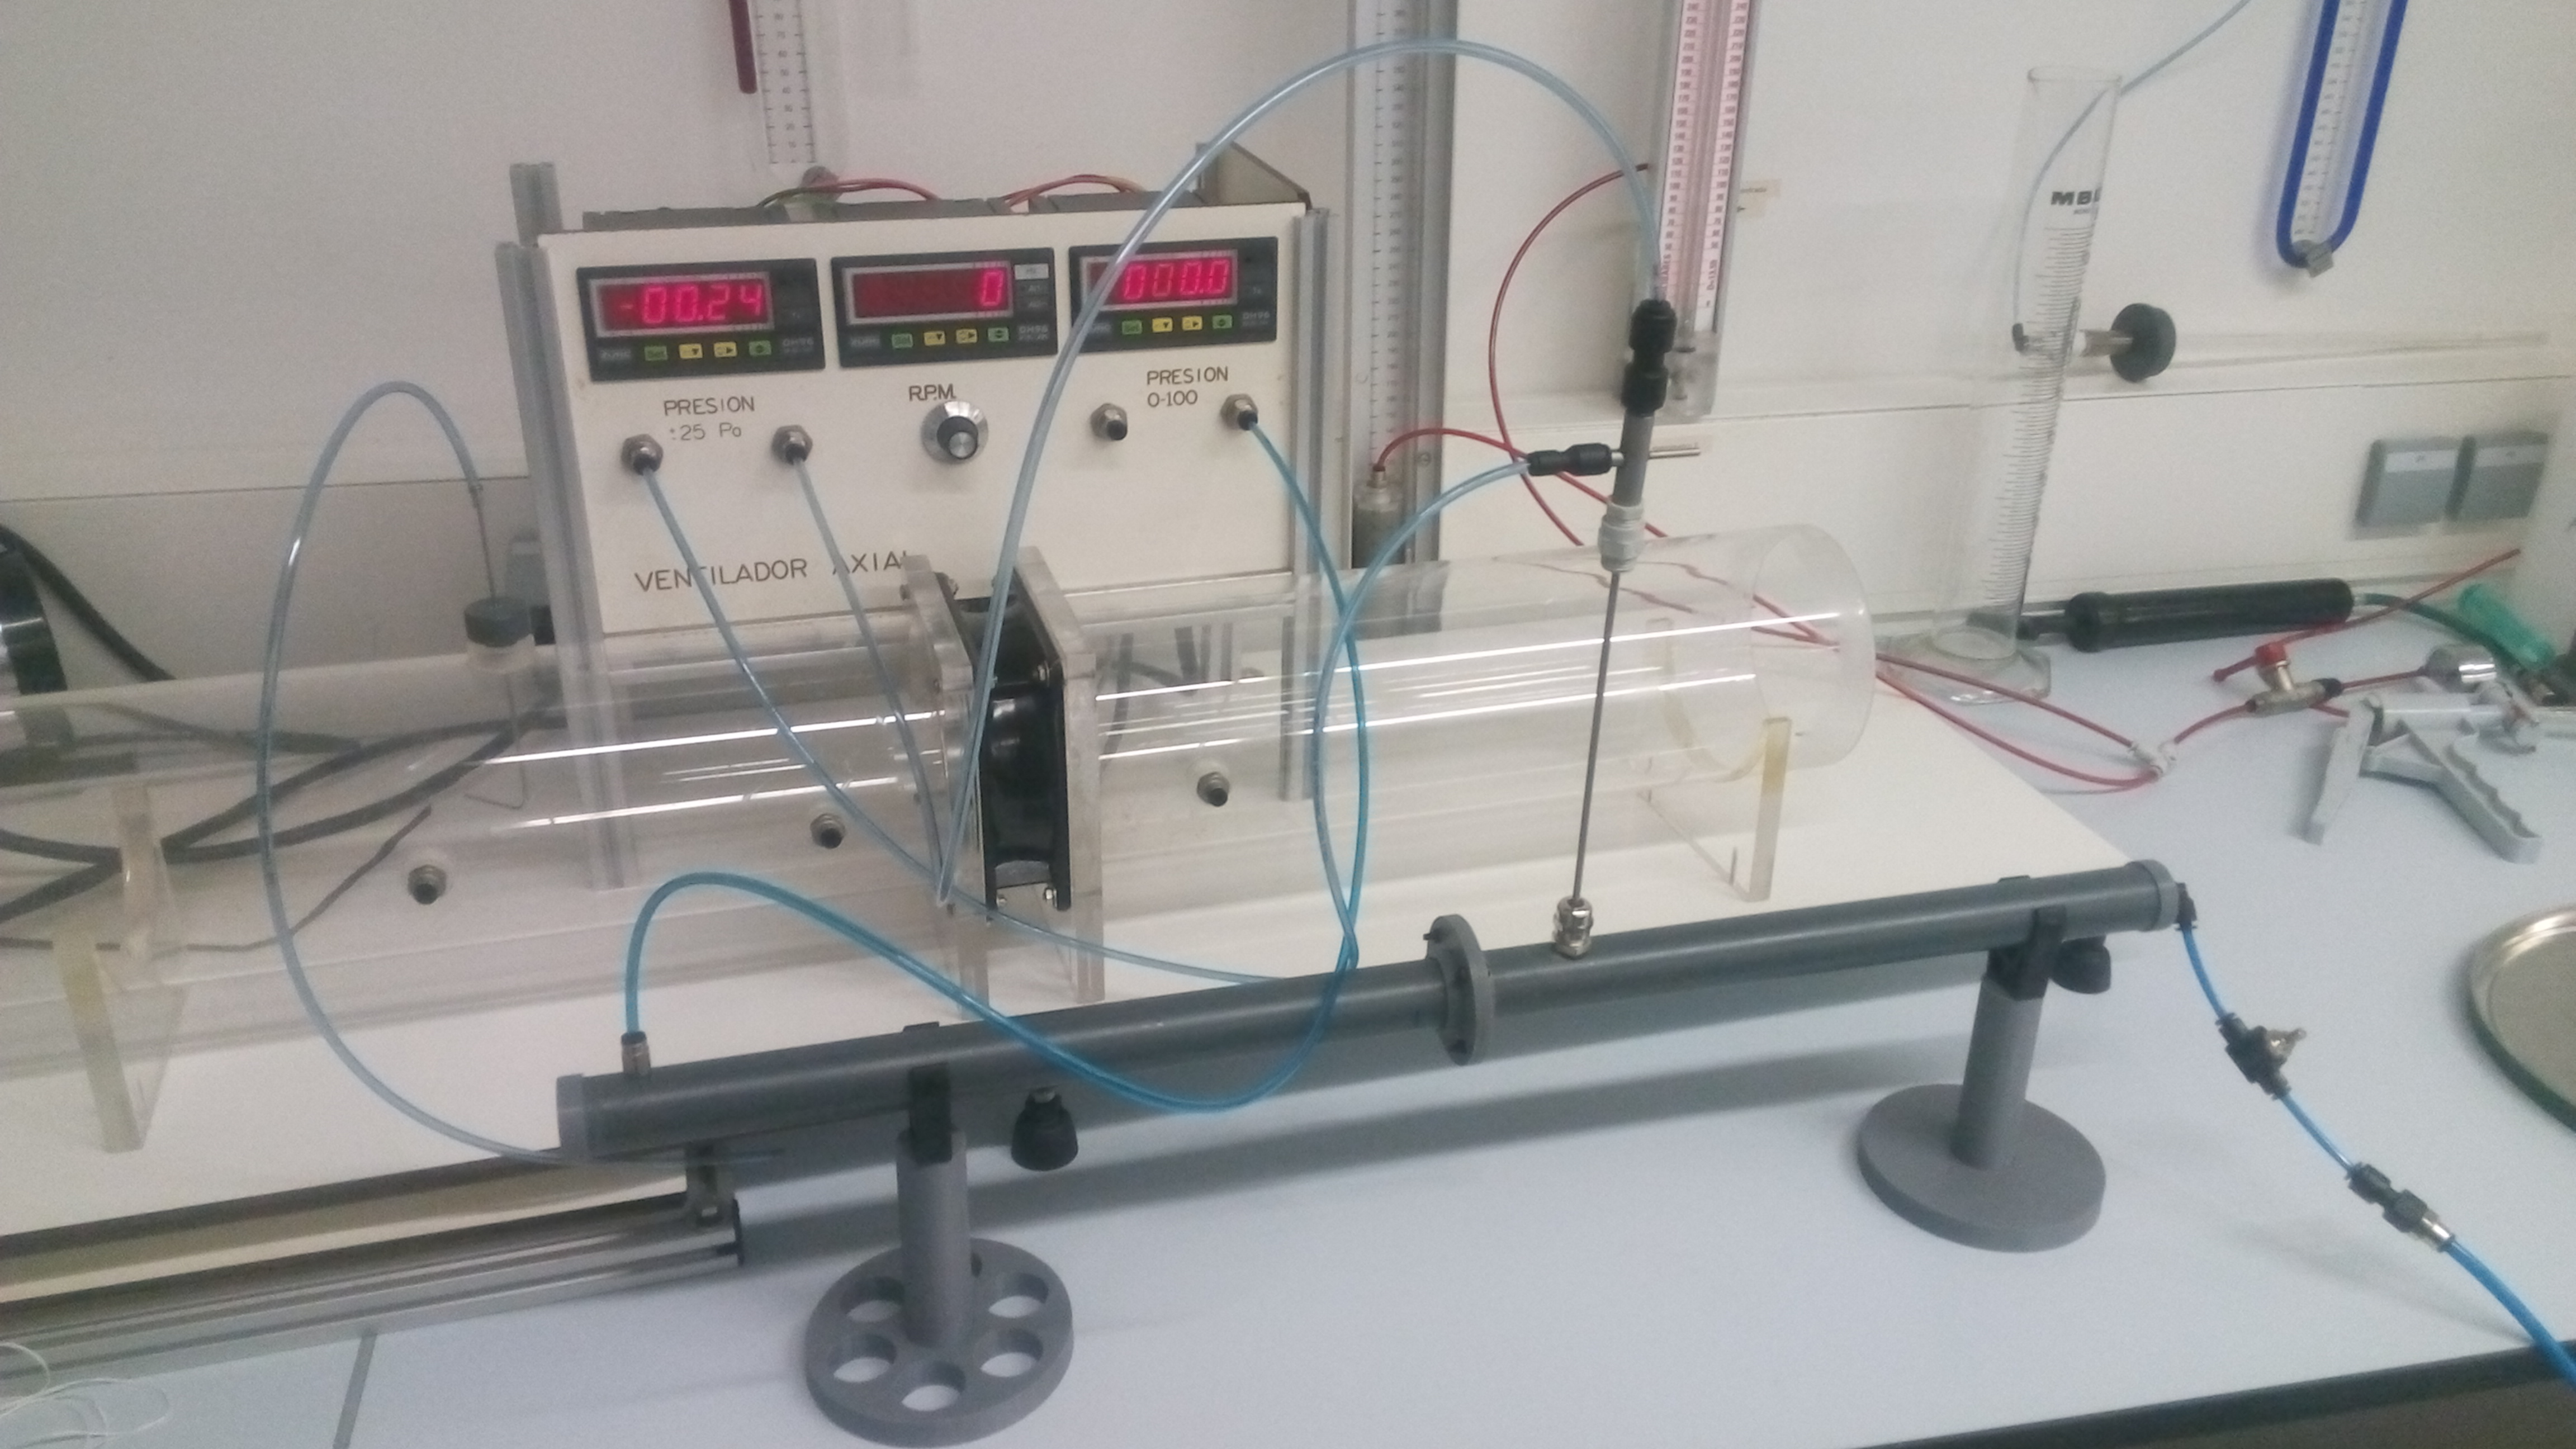
\includegraphics[width=0.8\linewidth]{M5inyector.jpg}
\caption[Caracterización del diafragma con inyector de aire a presión]{Ensayo de la Caracterización del diafragma con inyector de aire a presión, Método 5}
\label{fig:M5inyector}
\end{figure}

Se conectan las salidas del tubo de Prandtl, tal y como se ha detallado
para el método anterior, al instrumento para medir la presión entre el
rango \(\pm 25Pa\). En cambio la presión estática se conecta al medidor
de presión entre \((0-100)Pa\), siendo ésta la que alcanza un mayor
valor.

\subsubsection{Datos y Lecturas}\label{header-n467}

Los datos de entrada y los cálculos para obtener las variables
desconocidas, corresponden a los definidos para el método anterior. En
esta ocasión, al disponer de un regulador del caudal de entrada de aire
a presión, manejado a mano, la intensidad máxima estará limitada por el
rango de presiones que el instrumento de medida es capaz de ofrecer.
Siendo para la presión manométrica medida aguas arriba del diafragma de
\(100Pa\) y de \(\pm 25 Pa\), para la presión dinámica extraída del tubo
de Prandtl. A partir de estos máximos, se reduce progresivamente hasta
tener alrededor de 10 lecturas.

Se repiten estas pruebas para los diafragmas de 13mm (\autoref{tab:tablaM5d13}), 14mm (\autoref{tab:tablaM5d14}), 15,5mm (\autoref{tab:tablaM5d15}) y 16mm (\autoref{tab:tablaM5d16}); y se aunan los resultados en una misma gráfica.

\begin{table}[hb]
\centering
\caption[Valores para el diafragma de $13mm$]{Valores para el diafragma de 13mm, con una relación de áreas de $m=0,44$}
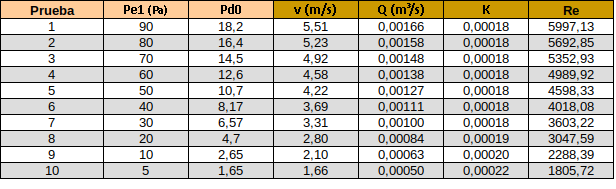
\includegraphics[width=0.85\linewidth]{tablaM5d13.png}
\label{tab:tablaM5d13}
\end{table}

\begin{table}
\centering
\caption[Valores para el diafragma de $14mm$]{Valores para el diafragma de 14mm, con una relación de áreas de $m=0,51$}
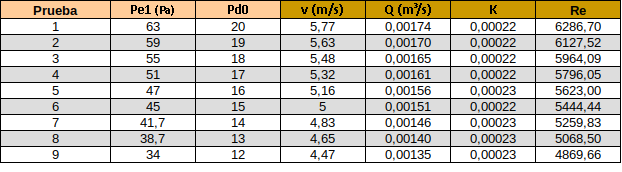
\includegraphics[width=0.85\linewidth]{tablaM5d14.png}
\label{tab:tablaM5d14}
\end{table}

\begin{table}
\centering
\caption[Valores para el diafragma de $15,5mm$]{Valores para el diafragma de 15,5mm, con una relación de áreas de $m=0,63$}
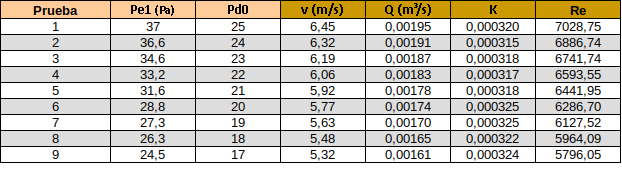
\includegraphics[width=0.85\linewidth]{tablaM5d15c5.png}
\label{tab:tablaM5d15}
\end{table}

\begin{table}
\centering
\caption[Valores para el diafragma de $16mm$]{Valores para el diafragma de 16 mm, con una relación de áreas de $m=0,67$}
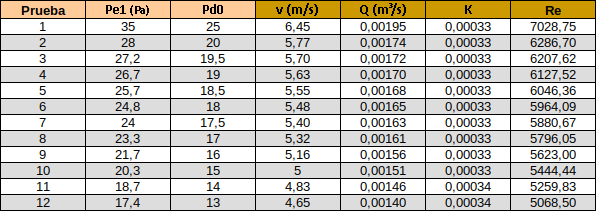
\includegraphics[width=0.85\linewidth]{tablaM5d16.png}
\label{tab:tablaM5d16}
\end{table}

\begin{figure}
\centering
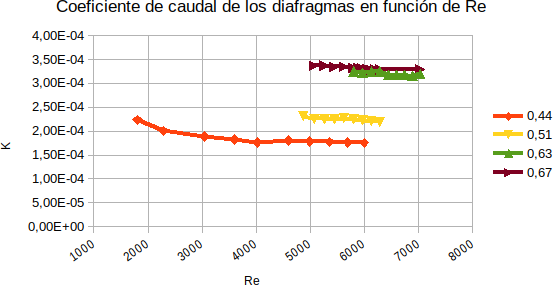
\includegraphics[width=0.75\linewidth]{grafM5.png}
\caption[Valores de coeficiente de descarga equivalente]{Valores de coeficiente de descarga equivalente respecto el número de Re, para los diafragmas 12'5, 13, 14, 15'5 y 16}
\label{fig:grafM5}
\end{figure}

\subsubsection{Conclusiones}\label{header-n498}

De la gráfica \autoref{fig:grafM5}, hallada mediante este método, se podrá obtener el
valor correspondiente del \emph{coeficiente de descarga equivalente}
para cada diafragma en función del número de Reynolds en el que se esté
trabajando.

A partir de la lectura de la presión aguas arriba del diafragma y con
este coeficiente, se podrá hallar el caudal y la potencia del ensayo
final en el canal, resolviendo las ecuaciones desccritas para el método anterior en el subapartado \ref{header-n423}:

\begin{itemize}
\item
  \(Q=K\sqrt{P_1}\)
\item
  \(Pot= K\cdot P_1^{3/2}\)
\end{itemize}

El valor del coeficiente permanece prácticamente constante, pero tras
consultar las gráficas normalizadas para ciertas placas planas en los
libros de \cite{Mataix82} o \cite{Miller96} se aprecia que esta
curva adquiere una mayor pendiente cuando se trabaja con números de Re
menores de 10³. No obstante, se puede mantener constante en un rango de
valores de Re, como es el caso. Además, como se va a utilizar el mismo
tubo para la chimenea del canal, con una presión estática comprendida en
el rango capturado, los valores hallados del experimento con el tubo de
Prandtl corresponderán a la velocidad de flujo que se obtendrá del
ensayo final del canal.

\section{Ensayo final}\label{header-n514}

\subsection{Definición}\label{header-n515}

Se disponen los equipos descritos anteriormente para llevar a cabo la
experimentación de la caída de una columna de agua, retenida por una
compuerta anidada a un pistón hidráulico, montado en una estructura
fijada al canal. Este colapso genera la ola que choca contra la pared de
una cámara, abierta por el fondo y sumergida. De forma que el nivel del
agua dentro de la cámara, se vea incrementada progresivamente. El
incremento de agua crea una corriente de aire, la cual en la realidad se
aprovecha para obtener energía con la colocación de unas turbinas WELLs.
En este caso se sustituye por una placa plana de diámetros
{[}13-14-15.5-16{]} mm.

Las condiciones iniciales o puesta en marcha, implica los siguientes
pasos:

\begin{enumerate}
\def\labelenumi{\arabic{enumi}.}
\item
  Se ajusta la posición de la compuerta a \(600mm\) del origen (el
  extremo del depósito de agua).
\item
  Colocar la parte de la tubería que contiene la toma piezométrica para
  la lectura de la presión estática aguas arriba del diafragma.
\item
  Conectar la salida de la toma al transductor de presión diferencial y
  este, a su vez, al ordenador, para que a traves de una tarjeta de
  adquisición se capture la presión estática aguas arriba del diafragma,
  tal y como se explica en el apartado \ref{header-n180} Chimenea.
\item
  La pared del fondo de la cámara se atornilla al fondo y la frontal se
  fija con una apertura de \(32mm\) para el paso del agua.
\item
  La condición incial del nivel de agua dentro del canal, se realiza con
  una bomba, regulando el caudal con una llave de paso, mencionado en el
  apartado \ref{header-n136} Canal y se establece de la siguiente manera:

  \begin{itemize}
  \item
    Llenado del canal entero hasta la altura de \(45mm\) en 'y', medida
    desde el fondo del canal.
  \item
    Tras cerrar la compuerta, se completa el llenado hasta la altura de
    \(145mm\), desde el mismo punto de referencia que el anterior.
  \end{itemize}
\end{enumerate}

\subsection{Datos y lecturas}\label{header-n544}

Por un lado, se graba la altura del nivel de agua alcanzada en la
cámara, con una regla colocada en el canal, ver \autoref{fig:Hd13}. Esta medida no varia en
exceso de una prueba a otra, ya que la condición inicial del volumen de
agua es la misma para todos los casos. Aunque, los diferentes diafragmas
provocarán que el llenado y el vaciado no se rijan en tiempos exactos,
en la siguiente imagen, se puede apreciar una altura media aproximada
alcanzada, estando entre 15-16 cm.

\begin{figure}[hb]
\centering
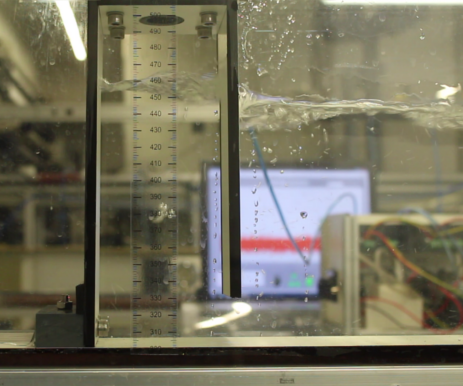
\includegraphics[width=0.6\linewidth]{Hd13.png}
\caption{Altura máxima alcanzada para el diafragma de diámetro de $13mm$}
\label{fig:Hd13}
\end{figure}

Por otro lado, la captura de la presión se realiza mediante el
transductor de presión, originalmente conectado a un \emph{display}. Sin
embargo, tal y como se explica en el apartado \ref{header-n180} Chimenea, el
objetivo de procesar los datos por ordenador es, principalmente, porque
por las simulaciones, se sabe que para captar el máximo valor de la
presión, el paso del tiempo como mínimo debe ser de \emph{0,05seg}, por
tanto se debe definir la captura del valor cada {[}ms{]}.

El programa realizado desde \emph{Ni LabVIEW 2015 SPI}, funciona de
forma interactiva con el usuario. Es decir, como se puede ver en
\autoref{fig:PTrj}, primero se selecciona ``Adquirir datos'', luego se
activa la subida de la compuerta y, finalmente, se detiene y se guardan
los resultados en un fichero ``.xls''. Estos archivos se exportan a
formato ``.csv'' para manipularlos y graficarlos mediante \emph{Octave}.

La adquisición de datos mediante sistemas digitales se realiza de forma
discreta, lo cual quiere decir que el resultado de la captura no es una
función continua. Es habitual utilizar un periodo de muestreo constante,
ya que esto facilita la reconstrucción de la misma. En este caso, el
periodo de muestreo utilizado es de 200us. En otras palabras, la
frecuencia de muestreo utilizada es de 5KHz (5000 muestras por segundo).

Dado que el control para la captura de los resultados de la presión
estática se realiza a mano, no se garantiza un retardo constante, desde
que empieza la lectura hasta accionar la apertura de la compuerta, para
todos los experimentos. No obstante, el interés se centra en conocer el
máximo valor alcanzado, el cual se da cuando el agua entra a la cámara.

Luego, a partir de \emph{Octave} se realiza una función para hallar los
valores que incluyan la presión máxima alcanzada, hasta que el
instrumento de medida no aprecie variaciones notables. Es decir, esta
curva no representa la subida y bajada del agua, sino cuándo se obtiene
el mayor impulso, que ocurre en el momento en que la ola entra en la
cámara (pasando p.e. de 75000 muestras a 4000, en el caso del diafragma
de diámetro 14mm).

Además, de las simulaciones, se obtiene que aproximadamente esto ocurre
desde \((1,2-2)seg\), así que, esta variación de presiones, donde se
encuentra el máximo, se representa en un tiempo de \(0,8seg\). Para
convertir los rangos de las muestras a los tiempos de simulación, se
multiplica el número de muestras por el periodo de captura. Con todo esto, se obtienen los gráficos mostrados en \autoref{fig:PT_EXPvsCFD}. 

\begin{figure}
\centering
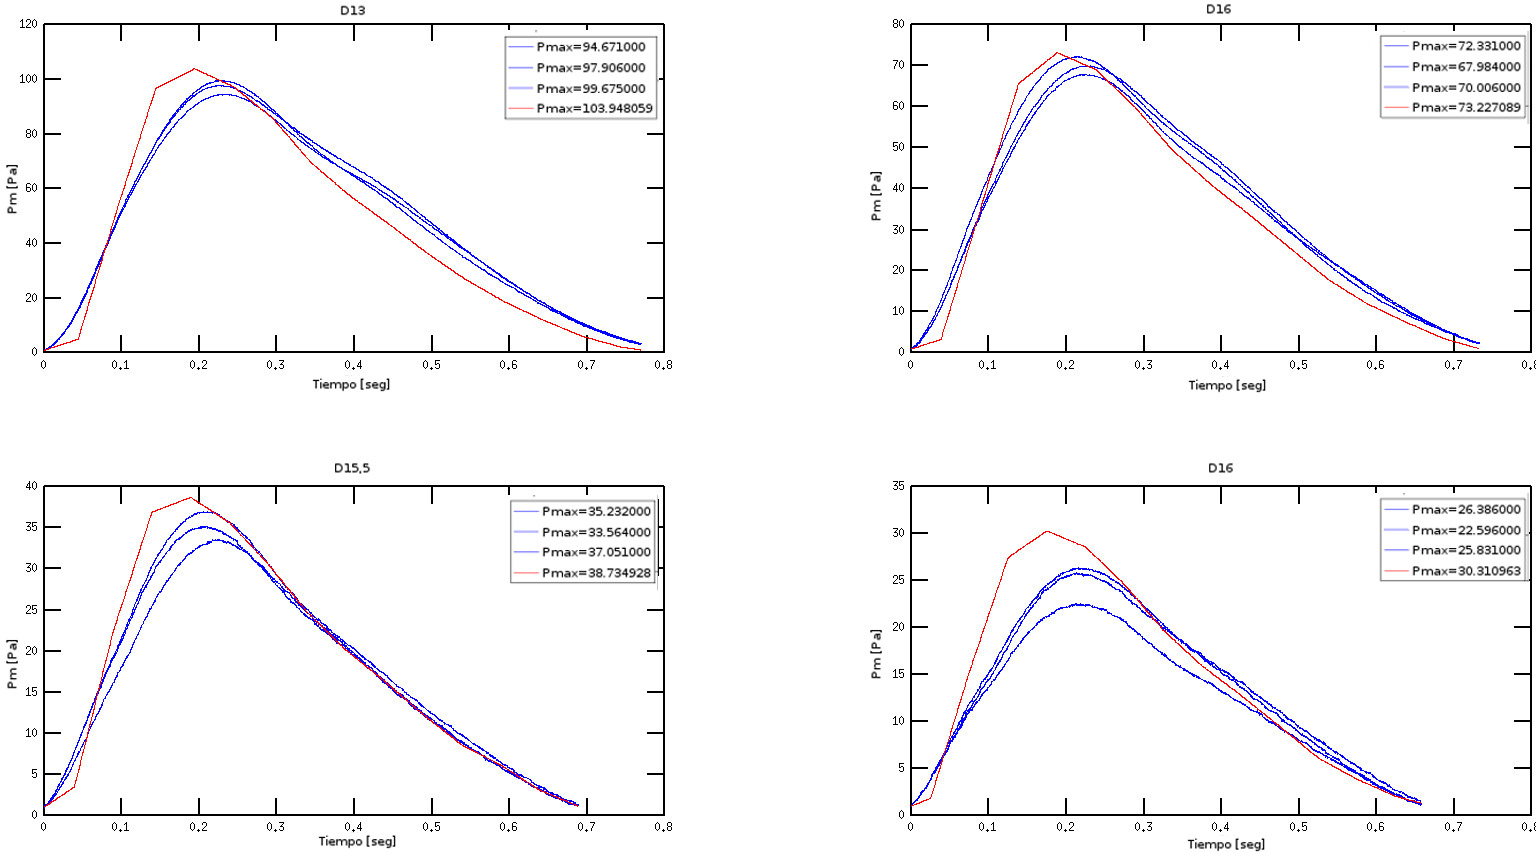
\includegraphics[width=\linewidth]{PT_EXPvsCFD.jpeg}
\caption[Resultados del ensayo y simulación]{Resultados del ensayo para las tres pruebas ensayadas más el resultado de la simulación}
\label{fig:PT_EXPvsCFD}
\end{figure}

También se realizan vídeos de la experimentación con cada diafragma, en
la \autoref{fig:nsyfinal} se tratan de capturar los instantes representados en
las simulaciones. De esta manera se puede comparar, de forma visible, la
dinámica del flujo de agua hallada mediante ambas vías. Esta
visualización podría mejorarse echando un tinte en el agua, o poniendo
un material opaco (p.e. papel) en la pared lateral del canal, de forma
que no se viera lo que hay detrás del canal y se apreciara mejor el
volumen de agua.

\begin{figure}
\centering
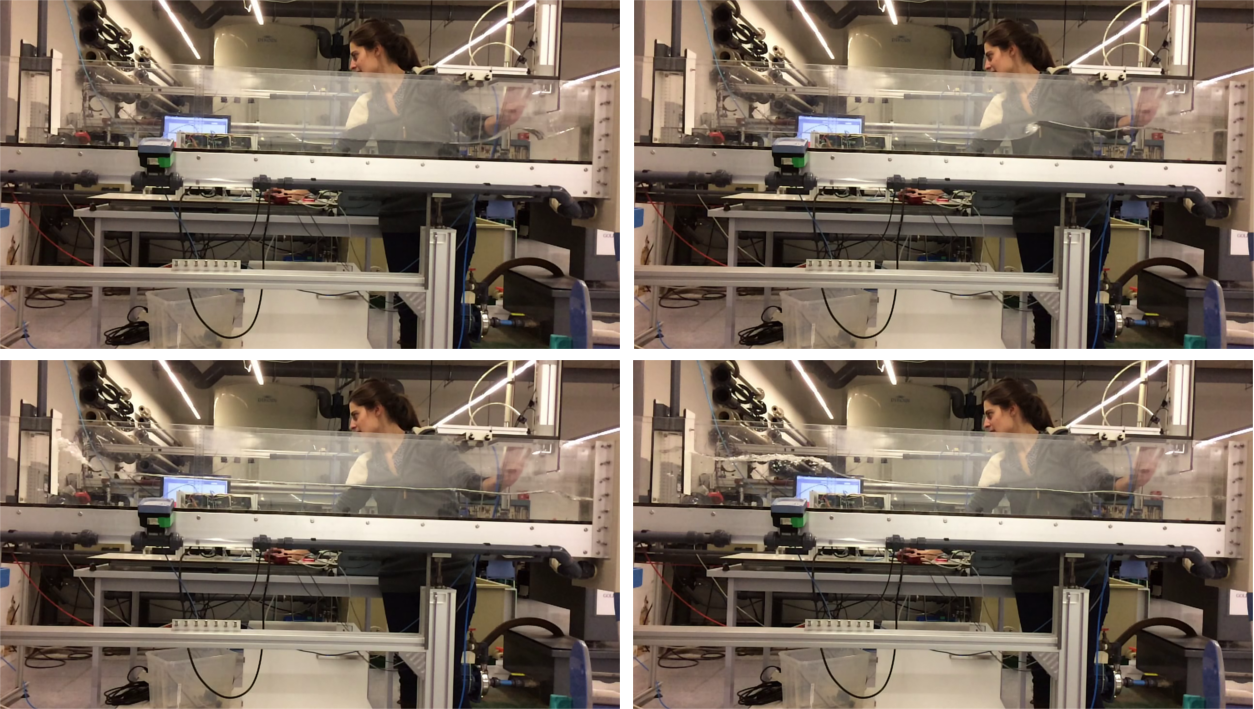
\includegraphics[width=\linewidth]{nsyFinal.png}
\caption{Representación del movimiento del flujo en el canal del laboratorio.}
\label{fig:nsyfinal}
\end{figure}

\subsection{Conclusiones}\label{header-n579}

Por un lado, tal y como se concluía en las simulaciones, no se aprecian
diferencias significativas en la altura del agua dentro de la cámara de
una prueba a otra. Asimismo, como se explica en el apartado 
\ref{header-n602} Cámara, está hallada con la vista y, aparte, la condición inicial del
llenado de agua es muy improbable que haya sido exacta para todas las
pruebas, por ello se toma una medida aproximada de \(15,5-16,5 cm\),
para todos los casos.

Principalmente, los datos que se extraen del experimento, con el objeto
de compararlos con los desarrollados computacionalmente, son los de la
diferencia de presiones a un lado y al otro del diafragma. Siendo
\(P_1\) la presión estática medida aguas arriba del diafragma y \(P_2\)
la presión atmosférica.

Tal y como se ha mencionado, los valores capturados a partir del ensayo
en el canal, no se han podido coger respetando el tiempo de simulación
de \(3seg\). Esto podría solucionarse con un microcontrolador, para
programar las señales y poder ejecutarlas en tiempo real (por un lado la
apertura de la compuerta y, por otro, el tiempo de captura de datos).
Aun así, se considera objeto de un proyecto de la rama de la
electronica, además, como se obtiene el valor de la presión máxima, a
partir de la caracterización del diafragma se podrán calcular las
variables de interés, resumidas en la \autoref{tab:nsycanal3d} que son el caudal y la potencia máximas.

\begin{table}[ht]
\centering
\caption[Caudal y potencia ensayo final]{Resultados del ensayo final, caudal y potencia para cada diafragma}
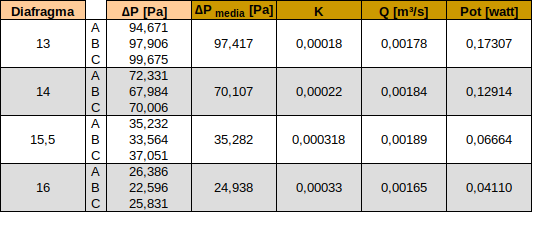
\includegraphics[width=0.7\linewidth]{tablaEnsayoCanal3D.png}
\label{tab:nsycanal3d}
\end{table}

\subsection{Presupuesto del ensayo}\label{header-n0}

Como ya se ha mencionado en el apartado de \autoref{header-n133} Descripción del equipamiento, los materiales utilizados para llevar a cabo la
experimentación son reutilizados de otras maquetas de ensayo o cedidos
por el colectivo de la UPV/EHU. Además de esto, se realizan dos facturas
a nombre del Departamento de Ingeniería Nuclear y Mecanica de los
Fluidos de la escuela de Ingeniería de Bilbao.

Es decir, los gastos que se computan en \autoref{presupuesto}, son cedidos
por la escuela de Ingeniería de Bilbao de la UPV/EHU.
Si se hubiera tenido que realizar de cero, el coste total estimado,
sumadas las horas de trabajo y precios de los diferentes materiales,
sería de $9375\euro{}$. Teniendo en cuenta que algunos precios pueden no
corresponder con el modelo exacto utilizado. Pues hay algunos materiales
que están descatalogados, pero se ha tratado de ajustar el modelo al más
análogo.

\begin{landscape}
\begin{longtable}[]{p{4cm}p{4cm}lllp{8cm}}
\caption{Presupuesto}
\label{presupuesto}
%\toprule
\hline
Tareas del proyecto & Elemento & Recurso & Unidades & Valor Unitario & Descripción\tabularnewline
\hline
%\midrule
\endfirsthead
\caption*{Presupuesto}
\hline
Tareas del proyecto & Elemento & Recurso & Unidades & Valor Unitario & Descripción\tabularnewline
\hline
\endhead
Maqueta de ensayo & Estructura del canal & M & 1 & 4000\euro{} & \href{http://dikoin.com/pdf/ENGLISH/FL\%2005.1.pdf}{Canal
Hidrodinámico 2,5m}.\tabularnewline
Apertura de la compuerta & Pistón hidráulico & M & 1 & 100\euro{} & Serie 453 de doble vástago y carrera de 160mm, ISO 15552.\tabularnewline
\multirow{2}{4cm}{Estructura soporte del Pistón} & \multirow{2}{4cm}{Placa policarbonato} & M & 1 & 15\euro{}/m & \multirow{2}{8cm}{Plancha perforada para anidar el pistón, y otra para ajustarlo al canal.}\tabularnewline
 & & L & 15 & 50\euro{}/h & \tabularnewline
\multirow{2}{4cm}{Compuerta} & \multirow{2}{4cm}{Placa policarbonato, juntas de goma} & M & 1 & 15\euro{}/m & \multirow{2}{8cm}{Plancha ranurada para introducir las juntas de goma.}\tabularnewline
 & & L & 4 & 50\euro{}/h & \tabularnewline
\multirow{2}{4cm}{Estructura OWC} & \multirow{2}{4cm}{Placa policarbonato, tacos} & M & 1 & 15\euro{}/m & \multirow{2}{8cm}{Tres planchas, dos hacen de pared y la tercera la parte superior con un agujero de salida.}\tabularnewline
 & & L & 20 & 50\euro{}/h & \tabularnewline
\multirow{2}{4cm}{Chimenea} & \multirow{2}{4cm}{Tubería} & M & 1 & 5\euro{}/m & \multirow{2}{8cm}{Tubería L=250 mm Dint=19,6mm.}\tabularnewline
 & & L & 3 & 50\euro{}/h & \tabularnewline
Impresiones 3D & Impresora 3D & M & 1 & 300\euro{} & Prusa i3.\tabularnewline
\multirow{2}{4cm}{Material de impresión} & \multirow{2}{4cm}{Plástico (PLA), diseños} & M & 1 & 12\euro{} & \multirow{2}{8cm}{\href{https://www.modpc.com/articulo/I610/filamento-3d-pla-bq-1-75mm-gris-ceniza-300gr}{Filamento 3D PLA 1,75mm gris ceniza}}.\tabularnewline
 & & L & 15 & 50\euro{}/h & \tabularnewline
Generación del flujo en conductos & Ventilador V003 & M & 1 & 5\euro{} & Tamaño (40x40)mm, caudal de 8,53CFM, 12V DC
0,09A, para la caracterización de diafragmas.\tabularnewline
Alimentación V003 regulable & Fuente de alimentación & M & 1 & 50\euro{} & Voltaje de salida de 0 a 15 VDC, para alimentar el
ventilador.\tabularnewline
Medición del la velocidad del flujo & Anemómetro & M & 1 & 600\euro{} & Modelo HTA4200, medidor de la velocidad del flujo.\tabularnewline
\multirow{2}{4cm}{Medida de la presión} & \multirow{2}{4cm}{Tomas de presión y presostatos} & M & 2 & 2\euro{} & \multirow{2}{8cm}{Perforaciones roscadas en la tubería de ensayo.}\tabularnewline
 & & L & 0.5 & 50 \euro{}/h & \tabularnewline
Captura de la presión por ordenador & Transductor de potencia & M & 2 & 80\euro{} & Modelo 267, serie 1173078, rango de medición de \(0-100 Pa\) y de \(\pm 25 Pa\).\tabularnewline
\multirow{2}{4cm}{Adquisición de datos} & \multirow{2}{4cm}{Conexión de una tarjeta de adqusición} & M & 1 & 100\euro{} & \multirow{2}{8cm}{\href{https://labjack.com/products/u3}{Labjack U3-LV}.}\tabularnewline
 & & L & 10 & 50\euro{}/h & \tabularnewline
Herramienta para el procesado & Ordenador & M & 1 & 700\euro{} & Control de adquisición de datos.\tabularnewline
\multirow{2}{4cm}{Programación de la adqusicion de datos} & \multirow{2}{*}{LabVIEW} & I & 1 & 1000\euro{} & \multirow{2}{8cm}{\href{https://www.ehu.eus/documents/1870470/3788660/software-relacion-es.pdf/a8683d42-8d3f-168a-8029-d1d18a14c8c2}{Licencia corporativa gratuita para equipos propiedad UPV/EHU}.}\tabularnewline
 & & L & 1 & 50\euro{}/h & \tabularnewline

Grabación del ensayo & Cámara de vídeo & M & 1 & 200\euro{} & Video Full HD, 16 Megapixeles, tarjeta LCD.\tabularnewline
Preparación de la grabación & Trípode & M & 2 & 30\euro{} & Se utiliza un trípode 106,5 cm de aluminio.\tabularnewline
\hline
%\bottomrule
\multirow{2}{8cm}{Total} & & M& & 6000& \tabularnewline
 & & L& 67,5h& 3375& \tabularnewline
\hline
\end{longtable}
M: Material L: Labor I: Licencia
\end{landscape}



